\chapter{Planificación e seguimento}
\minitoc
% \label{chap:Planificacioneseguimento}
% \vspace{0.5cm}

%%%%%%%%%%%%%%%%%%%%%%%%%%%%%%%%%%%%%%%%%%%%%%%%%%%%%%%%%%%%%%%%%%%%%%%%%%%%%%%%
% Objetivo:                        %
%%%%%%%%%%%%%%%%%%%%%%%%%%%%%%%%%%%%%%%%%%%%%%%%%%%%%%%%%%%%%%%%%%%%%%%%%%%%%%%%

  \lettrine{N}{este} capítulo detallaremos a planificación e o seguimento 
do proxecto, un proxecto que por diversas circunstancias se dividiu 
principalmente en tres grandes etapas, as dúas primeiras mentres VACmatch era 
unha iniciativa emprendedora baseada nun proxecto software libre e a última 
durante a cal se comezou unha conversión da iniciativa cara un proxecto 
comunitario.

  Durante o desenvolvemento xuridiron tamén diversos acontecementos 
relacionados co proxecto que tamén é importante resaltar debido a súa 
influencia no desenvolvemento e que se comentan durante este capítulo.

  \begin{description}
    \item [Agosto 2015 - Outubro 2015] VACmatch. Validación de negocio.
    \item [Outubro 2015 - Xaneiro 2016] VACmatch. Desenvolvemento de produto.
    \item [Xaneiro 2016 - Xuño 2016] De empresa a comunidade.
  \end{description}


  \section{Validación de negocio (Xullo 2015 -- Novembro 2015)}
  A duración desta etapa é de aproximadamente 4 meses e ven determinada polos 
primeiros pasos de VACmatch como iniciativa empresarial e que levan a orientar 
o desenvolvemento do produto cara o cliente, comezando cunha serie de 
prototipos para coñecer as suas necesidades e validar a idea de 
negocio.

  Durante o primeiro mes planifícase a realización dun prototipo visual co 
fin de comprobar a usabilidade e consolidar os requisitos dos clientes.
  De seguido, plantéxase crear un pequeno prototipo funcional, un 
MVP\footnote{\emph{Mínimo 
Producto Viable}} na metodoloxía Lean Startup, co obxectivo de testear as 
necesidades dos clientes e definir o produto final a desenvolver.

  En total realízanse dúas versións do prototipo da aplicación que son 
analizadas a continuación.

    \subsection{Prototipo visual}

      \subsubsection{Planificación e definición da iteración}
      Esta iteración dura un total de 4 semanas de desenvolvemento entre o 15 
de Xullo e o 16 de Agosto e realizase unha visita semanal ao cliente para obter 
feedback e mostrarlle a evolución do prototipo.

      Durante este periodo planificouse o desenvolvemento dunha aplicación moi 
sinxela e sen funcionalidade, que únicamente permitise analizar a usabilidade do 
sistema e comprobar se é factible adaptar o proceso de creación de un acta 
deportiva nunha aplicación móbil.

    Así mesmo, ao longo do período realizaranse ata tres visitas á federación 
coa que se traballou dende o primeiro momento para comprobar a experiencia de 
un futuro usuario real da aplicación e obter feedback para futuras melloras.

      \subsubsection{Revisión e feedback}
      Durante as visitas as federacións obtivéronse diversas prospostas que 
levaron a adaptar o prototipo, algunhas das cales se mencionan a continuación:

      \begin{itemize}
        \item Facer interactiva a aplicación e non mostrar grandes táboas con 
datos.
        \item Todas as accións deben xirar ao redor da acta.
        \item Crear partidos cando non hai cobertura.
      \end{itemize}

      \subsubsection{Tarefas e seguimento}

      A descomposición das tarefas desta iteración son as seguintes:

      \begin{description}
        \item [V.1] Crear esqueleto da aplicación.
        \item [V.2] Como árbitro quero poder consultar as próximas actas a 
cubrir.
        \item [V.3] Como árbitro quero poder consultar as actas xa cubertas.
        \item [V.4] Como árbitro quero poder editar un acta.
        \item [V.5] Como árbitro quero poder ver un acta.
        \item [V.6] Como árbitro quero poder ver os xogadores de ambos equipos.
        \item [V.7] Como árbitro quero poder engadir un evento.
        \item [V.8] Como árbitro quero poder rematar ou suspender un partido.
        \item [V.9] Como árbitro quero poder logearme.
        \item [V.10] Como árbitro quero poder seleccionar cales xogadores de 
cada equipo se atopan no encontro.
        \item [V.11] Como árbitro quero poder borrar un evento.
        \item [V.12] Estudio sobre React e Flux.
       \end{description}

       Para o desenvolvemento desta primeira versión do prototipo 
planificáronse 80 horas e puidéronse realizar tódalas tarefas no tempo indicado.

    \subsection{MVP funcional}

      \subsubsection{Planificación e definición da iteración}
      Esta iteración dura un total de 3 meses e desenvólvese entre o 16 de 
Agosto e o 15 de Novembro, realizando múltiples visitas a federacións e 
asociacións deportivas.

      Unha vez finalizadas as probas visuais e de usabilidade procédese 
a planificar o desenvolvemento para adaptar o prototipo e engadirlle 
funcionalidade sinxela, sen validacións e sen funcionalidade offline, co 
obxectivo de obter un prototipo funcional que poida ser utilizado por usuarios 
reais nun entorno controlado.

      Engadirase funcionalidade para as vistas creadas na iteración anterior, 
comezando polo listado de actas pendentes e rematadas e diversos compoñentes 
xenéricos como os que se utilizan para listar xogadores e outros elementos como 
poden ser as actas.

      Únicamente se engadirá a funcionalidade básica imprescindible para 
xestionar un encontro, excluindo requisitos como a sinatura de actas ou a 
creación offline das mesmas co fin de axilizar as primeiras probas.

      Durante a iteración tamén se farán visitas á federación para mostrar o 
estado do desenvolvemento e para buscar que tamén árbitros reais vexan os 
progresos e proporcionen feedback.

      Unha vez rematada a iteración realizarase o torneo onde probar o 
prototipo desenvolto nun caso real; pódese ver o desenvolvemento de dita 
competición na Sección~\ref{sec:torneo_vacmatch}.

      \subsubsection{Revisión e feedback}
      Durante as visitas as federacións obtivéronse múltiples propostas e 
melloras, moitas das cales será incorporadas ao backlog do proxecto mentres que 
outras serán rexeitadas polo momento ao non considerarse prioritarias ou por 
ser casos de usos moi concretos para esa federación e dificilmente 
extrapolables a outras.

      \textbf{Listaxe de tarefas engadidas ao backlog}.
        \begin{itemize}
          \item Meter xogadores manualmente xa que poden non terse creado no 
sistema de xestión.
          \item Poder ver os eventos de forma sinxela dende a vista de fin de 
partido para que os equipos vexan o que están asinando.
         \item Editar dorsal dos xogadores xa que poden cambiar.
         \item Ter opción de non poñer motivo para as tarxetas.
         \item Mostrar foto de xogador ao engadir un evento.
        \end{itemize}

      \textbf{Listaxe de tarefas rexeitadas polo momento}.
        \begin{itemize}
         \item Ao marcar doble amarela, avisar da expulsión. Moi concreta para 
un deporte, non se implementa de momento.
         \item Mostrar confirmación de que se engadíu un evento.
         \item Avisar aos delegados/personal do clube cando se sube un acta.
         \item Posibilidade de que o árbitro engada un anexo na casa á acta en 
lugar de escribir as incidencias.
        \end{itemize}

      \subsubsection{Tarefas e seguimento}

      As tarefas que se realizarán durante esta iteración son as seguintes:

        \begin{description}
        \item [MVP1] Como árbitro quero poder cargar a lista de actas pendentes.
        \item [MVP2] Como árbitro quero poder cargar a lista de actas rematadas.
        \item [MVP3]Como árbitro quero poder ver os datos dun partido.
        \item [MVP4]Como árbitro quero poder ver a lista de xogadores dun 
equipo.
        \item [MVP5] Como árbitro quero poder seleccionar os xogadores 
presentes no partido.
        \item [MVP6] Como árbitro quero poder engadir un gol a un xogador.
        \item [MVP7] Como árbitro quero poder engadir unha falta a un xogador.
        \item [MVP8] Como árbitro quero poder engadir unha tarxeta (amarela ou 
vermella) a un xogador.
        \item [MVP9] Como árbitro quero poder ver a lista de eventos de un 
partido.
        \item [MVP10] Como árbitro quero poder borrar eventos de un partido.
        \item [MVP11] Como árbitro quero poder engadir incidencias a un partido.
       \end{description}

      Planificouse un total de 65 horas para desenvolver esta iteración que non 
resultaron suficientes, obrigando a facer un total de 10,5 horas extra motivado 
polo descoñecemento da tecnoloxía, de forma que foi preciso invertir un maior 
número de horas das esperadas en formación.

    \subsubsection{I Torneo VACmatch}
    \label{sec:torneo_vacmatch}
    Durante este periodo tamén se planificou a organización dun torneo de 
  fútbol sala a finais do mes de Outubro coa idea de probar nun entorno real 
  e controlado, os primeiros prototipos desenvoltos.

  Finalmente participaron 6 equipos e mais de 50 persoas durante os dóus días 
que durou o evento, obtendo todo tipo de suxerencias e detectando múltiples 
erros que serán analizados e comentados na seguinte iteración.

  \begin{figure}[h!]
        \begin{center}
        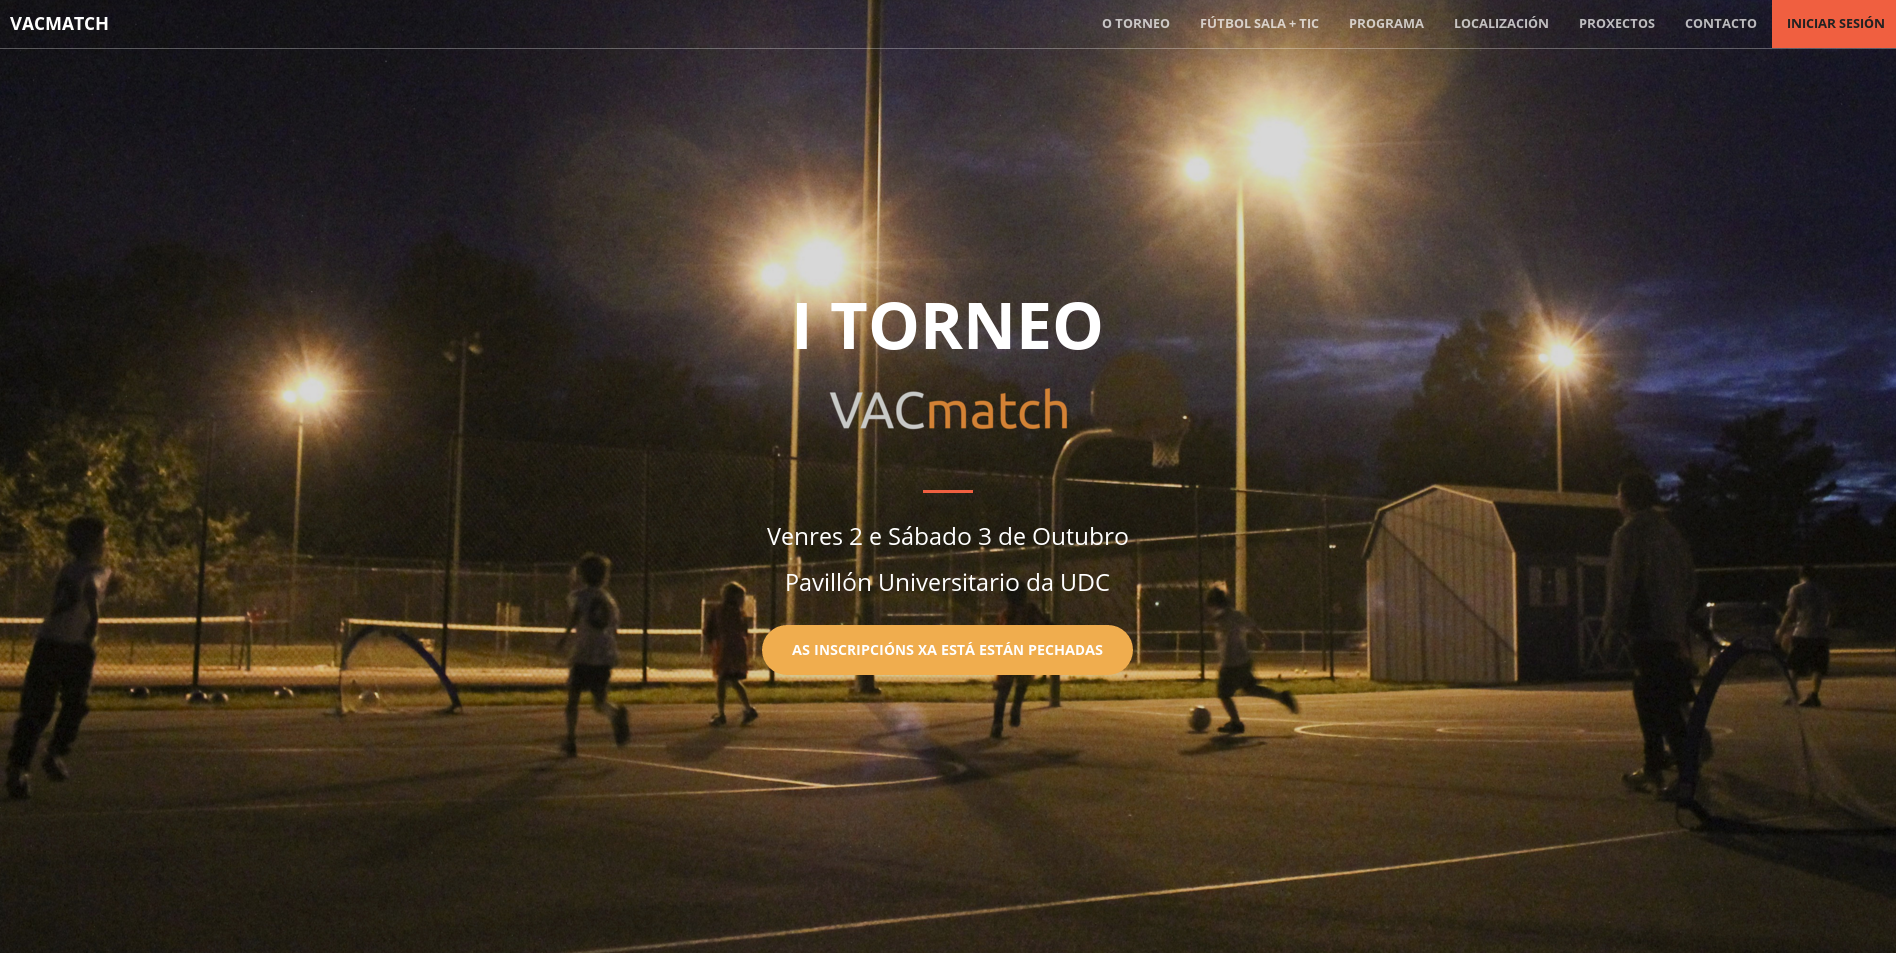
\includegraphics[width=\textwidth]{./img/torneo_vacmatch.png}
        \caption{Web do I Torneo VACmatch}
        \end{center}
  \end{figure}
\
  \section{Desenvolvemento de produto (Novembro 2015 -- Xaneiro 2016)}
  Tras analizar os problemas e os erros cometidos durante a realización do I 
Torneo VACmatch, e concretamente no funcionamento da aplicación móbil durante o 
mesmo, decidíuse comezar novamente dende o principio un proxecto novo en lugar 
de facer unha refactorización do prototipo.

    Durante este tempo decidimos inscribir o proxecto no ``Concurso 
Universitario de Software Libre'' o que incentivou a comezar a escribir un 
blog técnico, a través da conta de Medium\footnote{Medium é unha rede social 
que permite crear e seguir blogs de múltiples temáticas} de VACmatch, no que 
contar os avances que suceden durante o desenvolvemento do proxecto.

  Neste periodo de 3 meses de duración planifícase adicar unha media de 4 
horas diarias en VACmatch Mobile debido a que en paralelo se está a traballar 
na versión de VACmatch Web.

  Así mesmo, descontando os múltiples días festivos, calcúlase un total de 208 
horas de traballo divididas en 5 iteracións.

    \subsection{1ª e 2º iteración. Creación do proxecto e xestión de actas}

      \subsubsection{Planificación e definición da iteración}
      Estas iteracións transcorren ao longo do mes de Novembro, adicando 15 
dias a cada unha.

      A primeira céntrase en comezar o desenvolvemento da 
aplicación pensando dende o primeiro momento no funcionamento tanto online 
como offline e controlando os posibles conflictos que poidan suceder entre os 
datos.

      Comézase co estudo da tecnoloxía en profundidade xa que os 
prototipos non utilizaban nin Reflux nin PouchDB e simplemente enviaban os 
datos a un servizo web remoto.

      Crease tamén o proxecto base engadindo a licencia e defínese o modelo de 
datos, que vai cambiar bastante do modelo inicial, pensando para unha base de 
datos relacional que é a que podíamos atopar na API remota de VACmatch Web.

      É por iso que os datos serán desnormalizados e pasarán a almacenarse en 
documentos en lugar de en táboas.

      Por último comézase a implementación do listaxe de actas a cubrir e de un 
boton para engadilas e eliminalas de xeito sinxelo para facer as primeiras 
probas.

        Durante a 2º iteración planifícase o desenvolvemento das páxinas 
principais e básicas para a xestión da acta dun encontro.

      As funcionalidades que se abordarán neste sprint céntranse principalmente 
na vista na que se mostra o resumo actual da acta así como o control do tempo, 
co fin de permitir xestionar o encontro en tempo real de forma interactiva.

      \subsubsection{Revisión e feedback}
      Durante esta iteración analizáronse os problemas detectados durante o 
torneo, optando por comezar a implementación do proxecto dende cero como se 
comentou anteriormente.

      Tamén se realizaron diversas publicacións do blog para comentar a 
realización de dita competición e sobre todo analizar aspectos como a elección 
tecnolóxica, a metodoloxía de desenvolvemento e as próximas funcionalidades a 
abordar.

  Ao non realizar ningunha visita a federacións, non se obtivo o seu feedback.

      \subsubsection{Tarefas e seguimento}

      Durante estas iteracións realizáronse as seguintes tarefas que tamén 
se poden observar a través dos Diagramas de Gant~\ref{fig:gant01} e 
~\ref{fig:gant02}.

        \begin{description}
         \item [S1.1] Definir modelo de datos.
         \item [S1.2] Definir arquitectura e tecnoloxía.
         \item [S1.3] Deseñar mockups.
         \item [S1.4] Crear proxecto base.
         \item [S1.5] Crear modelos en PouchDB.
         \item [S1.6] Estudo da tecnoloxía. React, Reflux, PouchDB, Redmine
         \item [S1.7] Como árbitro quero poder obter a lista de actas a cubrir.
         \item [S1.8] Permitir crear e borrar actas para tarefas de test.
         \item [S1.9] Engadir licencia e Readme
         \item [S2.1] Como árbitro quero ver o resumo da acta.
         \item [S2.2] Como árbitro quero controlar o tempo do partido.
         \item [S2.3] Como árbitro quero manter o tempo do partido aínda que 
cambie de páxina.
         \end{description}

        \begin{figure}[h!]
          \begin{center}
          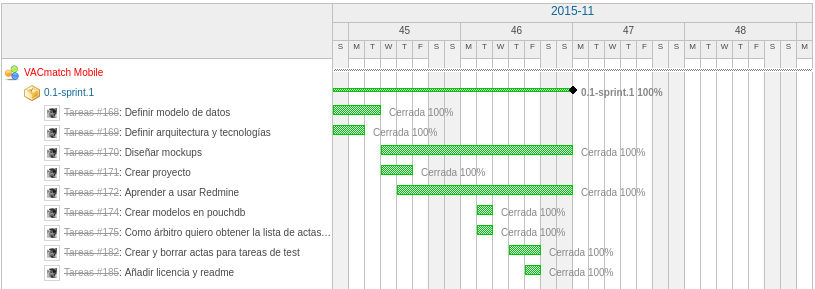
\includegraphics[width=\textwidth]{./img/gant_diagrams/01.png}
          \caption{Diagrama de Gant do sprint 1}
          \label{fig:gant01}
          \end{center}
        \end{figure}

        \begin{figure}[h!]
          \begin{center}
          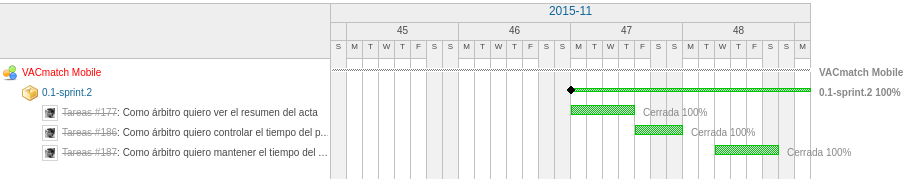
\includegraphics[width=\textwidth]{./img/gant_diagrams/02.png}
          \caption{Diagrama de Gant do sprint 2}
          \label{fig:gant02}
          \end{center}
        \end{figure}

  A planificación inicial de 71 horas de desenvolvemento finalmente cumpríuse 
correctamente, incluso reducindo o tempo empregado ata as 68.

    \subsubsection{Participación na I Lonxa de Financiamento Responsable}
    \label{sec:lonxa}
    Durante este tempo tamén cómpre destacar a participación de VACmatch na I 
Lonxa de Financiamento Responsable en Galicia, permitíndonos presentar o noso 
proxecto ante diversos inversores preocupados pola responsabilidade social das 
empresas.

    \begin{figure}[h!]
          \begin{center}
          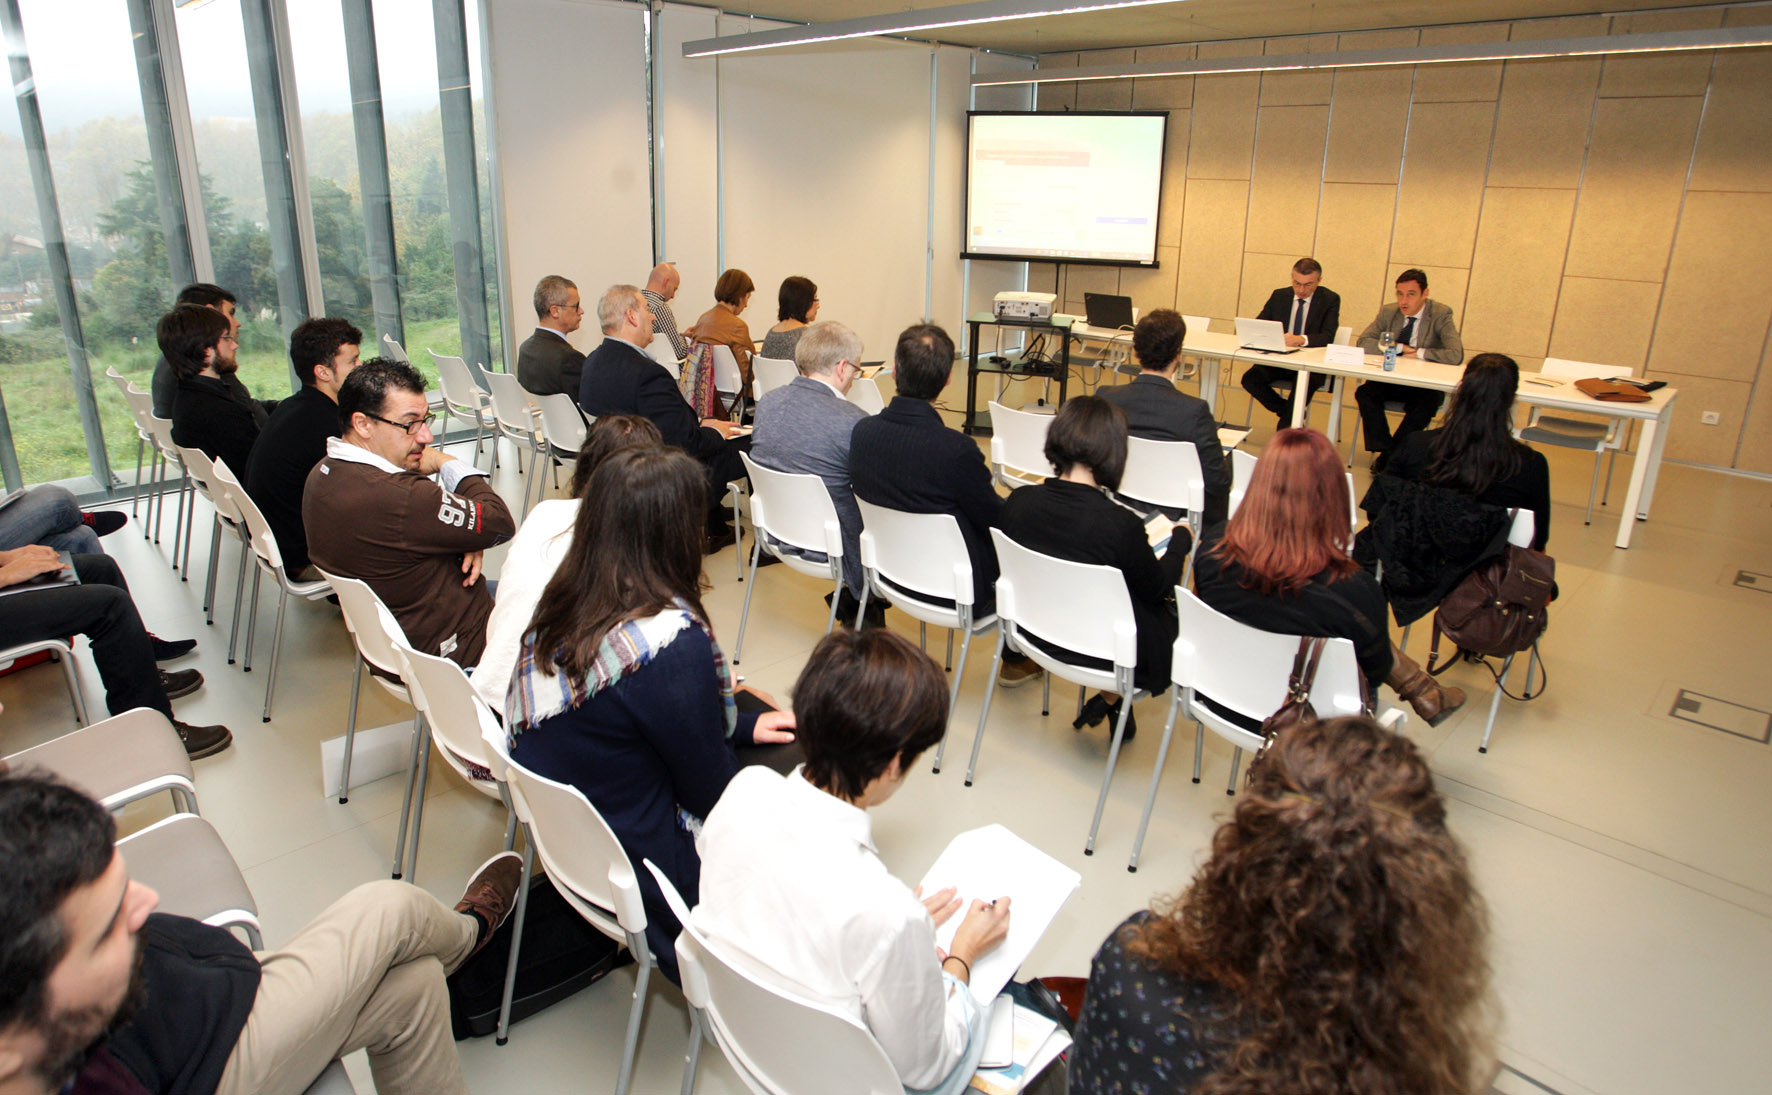
\includegraphics[width=0.8\textwidth]{./img/inversion_responsable.jpg}
          \caption{I Lonxa de Financiamento Responsable}
          \label{fig:lonxa}
          \end{center}
    \end{figure}

        Foi unha experiencia única que nos permitíu introducirnos por primeira 
vez no mundo da inversión en startups e coñecer aos diversos proxectos que se 
presentaron, obtendo tamén feedback dos asistentes e participantes.

    \subsection{3ª iteración. Eventos}

      \subsubsection{Planificación e definición da iteración}
      Esta iteración comeza o 30 de Novembro e remata o 13 de Decembro, unha 
iteración de dúas semanas de duración que se centrada principalmente na xestión 
de eventos dos encontros, tarefas que requiren unha forte planificación e 
análise xa que se busca que ditos eventos sexan o máis xenéricos posibles e 
facilmente adaptables aos diversos deportes.

      Da mesma forma plantéxase crear tipos de eventos que modifiquen tamén a 
propia acta, actualizando na mesma tanto o resultado como as faltas cometidas.

      Por último incorpórase tamén na iteración a posibilidade de convocar e 
editar persoas dun equipo así como algún pequeno erro detectado na última 
iteración.

      \subsubsection{Revisión e feedback}
      Esta iteración centróuse en avanzar a maior velocidade no 
desenvolvemento, pódese observar cómo o número de horas asignadas supera a 
media teórica planificada para o período completo.

      Non se realizou ningunha visita a federacións e centrouse prácticamente 
todo o esforzo, fora do desenvolvemento, en preparar a presentación para a I 
Lonxa de Financiamento Responsable en Galicia da que se falou 
anteriormente na Sección~\ref{sec:lonxa} e na que se obtiveron diversos 
comentarios para enfocar o modelo de negocio e o desenvolvemento da aplicación 
cara o cliente.

      \subsubsection{Tarefas e seguimento}

      A continuación móstranse as diversas tarefas realizadas na iteración e 
pódese ver o Diagrama de Gant correspondente na Figura~\ref{fig:gant03}:

        \begin{description}
          \item [S3.1] Como árbitro quero poder engadir un evento.
          \item [S3.1.1] Como árbitro quero ver a lista de xogadores para 
asignar un evento.
          \item [S3.1.2] Como árbitro quero poder confirmar engadir un evento.
          \item [S3.1.3] Como árbitro quero engadir unha causa a un evento.
          \item [S3.2] Cómo árbitro quero poder ver a lista de eventos de un 
partido.
          \item [S3.3] Como árbitro quero que se xeneren eventos de comezo e 
fin de partido.
          \item [S3.4] Como árbitro quero que se xeneren eventos ao cambiar de 
parte.
          \item [S3.5] Como árbitro quero que se actualice o resultado ao 
engadir un gol.
          \item [S3.6] Como árbitro quero que se actualicen as faltas 
automáticamente.
          \item [S3.7] Como árbitro quero poder convocar e desconvocar 
xogadores.
          \item [S3.8] Como árbitro quero poder cambiar o dorsal de un xogador 
nun partido determinado.
          \item [S3.9] Como árbitro quero poder borrar un evento.
          \item [S3.10] Como árbitro quero ver a lista de eventos de un partido 
ordenada por tempo e parte.
          \item [S3.11] Mostrar únicamente xogadores convocados ao engadir un 
evento.
          \item [S3.12] Como árbitro quero que ao borrar un evento se 
actualicen os 
resultados e as faltas na Acta.
          \item [S3.12] Erro: Cando non hai ningún evento de cambio de parte 
hai un error.
          \item [S3.13] Erro: Correxir erro cando se engade un evento con causa.
        \end{description}

        \begin{figure}[h!]
          \begin{center}
          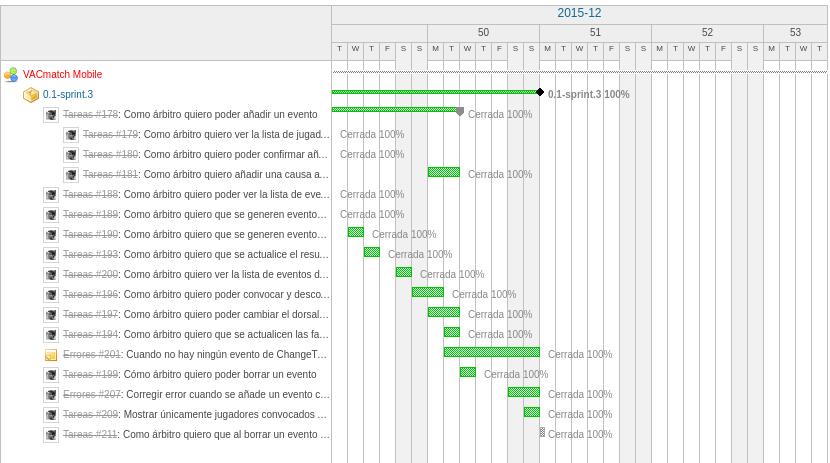
\includegraphics[width=\textwidth]{./img/gant_diagrams/03.png}
          \caption{Diagrama de Gant do sprint 3}
          \label{fig:gant03}
          \end{center}
        \end{figure}

        Finalmente a planificación inicial de 51 horas cumpríuse correctamente 
quedando un extra de 6 horas que foron reasignadas ao outro proxecto.

    \subsection{4ª iteración. Xestión de usuarios e creación offline de actas}

      \subsubsection{Planificación e definición da iteración}
      Esta iteración ten lugar entre o 14 e o 30 de Decembro de 2015 e céntrase 
na autenticación da aplicación que debe integrar unha base de datos remota para 
que os árbitros poidan conectarse co seu usuario e tamén inclúe a creación e 
edición manual de actas que en anteriores iteracións foi engadida únicamente 
para probas internas pero sen realizar as comprobacións necesarias.

      Tamén se planifican tarefas para comezar as primeiras partes da memoria 
do proxecto que incluen a introdución, o estado da arte e os fundamentos 
tecnolóxicos.

      \subsubsection{Revisión e feedback}
      Durante este periodo escribíuse unha nova entrada no blog do proxecto 
na que se fixo unha introdución aos fundamentos tecnolóxicos do mesmo, 
explicando a motivación da elección das tecnoloxías e mostrando un exemplo 
moi sinxelo.

      Por último mostrouse tamén a estrutura da aplicación e as partes máis 
importantes do proxecto, pensando en facilitar a introdución no 
desenvolvemento aos posibles interesados en colaborar no mesmo.

      \subsubsection{Tarefas e seguimento}

      O listado de tarefas abordadas durante esta iteración é o seguinte:

        \begin{description}
          \item [S4.1] Como usuario quero poder facer log in.
          \item [S4.2] Engadir diferenciación entre Persoal e Xogadores.
          \item [S4.3] Como usuario quero poder facer log out.
          \item [S4.4] Como árbitro quero poder crear un partido manualmente.
          \item [S4.5] [Memoria] Definir introdución.
          \item [S4.6] [Memoria] Estado da arte.
          \item [S4.7] [Memoria] Fundamentos tecnolóxicos.
          \item [S4.8] [Memoria] Engadir modelo.
          \item [S4.9] Como árbitro quero poder editar un acta creada dende o 
móbil.
          \item [S4.10] Erro: Correxir erro coa variable dialogIsOpen ao editar 
o dorsal dun xogador.
        \end{description}

        \begin{figure}[h!]
          \begin{center}
          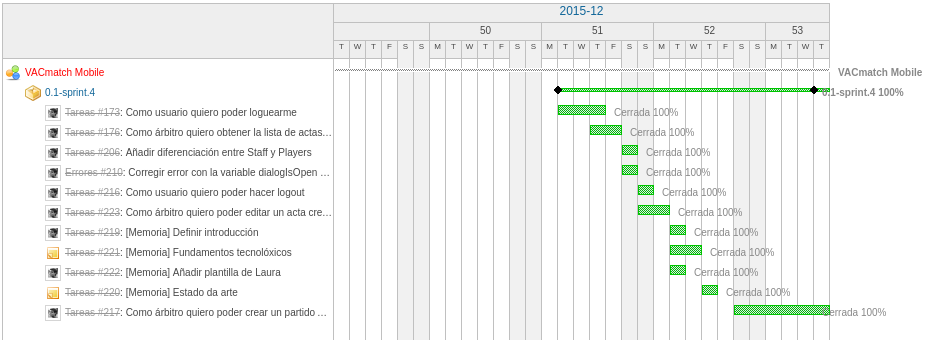
\includegraphics[width=\textwidth]{./img/gant_diagrams/04.png}
          \caption{Diagrama de Gant do sprint 4}
          \label{fig:gant04}
          \end{center}
        \end{figure}

      Esta vez a planificación non foi moi acertada debido a diversos 
imprevistos externos ao proxecto, o que levou a necesidade de mover diversas 
tarefas á seguinte iteración para axustar a planificación incial de 53.5 horas 
ata as 44 que se realizaron finalmente.

    \subsection{5ª iteración. Sinaturas}

      \subsubsection{Planificación e definición da iteración}
      Esta iteración comeza o día 1 de Xaneiro de 2016 e remata o día 8 
e centrase na última vista da aplicación, aquela que permite xestionar a 
finalización do encontro dando a posibilidade de asinar a acta e engadir 
comentarios por parte do árbitro.

      Na iteración anterior detectáronse varias melloras a incluir como facer 
que por defecto as contas creadas dende a aplicación móbil sexan todas de tipo 
árbitro. Así mesmo facer que se engada a dito usuario como árbitro do encontro 
en tódalas actas que cree esa conta.

      \subsubsection{Revisión e feedback}
      Ao finalizar esta iteración publicouse unha nova entrada no blog do 
proxecto expoñendo a metodoloxía áxil utilizada para o desenvolvemento, así 
como aquelas nas que se basea (Scrum e eXtreme Programming) e a metodoloxía de 
negocio orientada cara o cliente (Lean Startup).

      Por último tamén se publicou o fluxo de traballo que se realiza para 
contribuir ao proxecto co sistema de control de versións Git, co fin de 
facilitar o traballo a futuros contribuidores.

      \subsubsection{Tarefas e seguimento}

      Durante esta iteración realizáronse as seguintes tarefas e das cales se 
pode observar o seu diagrama de Gant na Figura~\ref{fig:gant05}.

        \begin{description}
         \item [S5.1] Como árbitro quero poder asinar un acta.
         \item [S5.2] Como árbitro quero que unha ou varias persoas convocadas 
de cada equipo poidan asinar un acta.
         \item [S5.3] Como árbitro quero poder engadir comentarios a un acta.
         \item [S5.4] Como árbitro quero poder borrar un xogador da lista de 
convocados.
         \item [S5.5] Crear un árbitro ao crear un novo usuario na aplicación 
móbil.
         \item [S5.6] Engadir o árbitro que ten o usuario asignado nas actas 
que crea.
        \end{description}

        \begin{figure}[h!]
          \begin{center}
          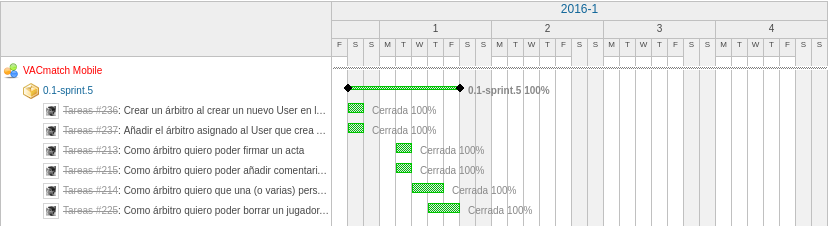
\includegraphics[width=\textwidth]{./img/gant_diagrams/05.png}
          \caption{Diagrama de Gant do sprint 5}
          \label{fig:gant05}
          \end{center}
        \end{figure}

        Nesta iteración a planificación incial de 32 horas foi sobrestimada 
polo que finalmente sobraron 5 horas de desenvolvemento que foron reasignadas 
ao outro proxecto.

  \section{De empresa a comunidade (Xaneiro 2016 -- Maio 2016)}
  Durante o mes de Xaneiro de 2016 decidíuse abandonar o proxecto de VACmatch 
como iniciativa empresarial por diversos motivos e continuar con él únicamente 
como proxecto comunitario de software libre.

  Motivado por isto, producíuse un parón de aproximadamente un mes de duración 
e ao mesmo tempo comezouse a traballar nunha empresa externa polo que durante 
este período diminuíu considerablemente o tempo dispoñible para continuar co 
proxecto.

  O número de horas total estimado para este período de 6 iteracións é de 189, 
todo nun total de 5 meses, o que supón unha media aproximada de 2 horas 
diarias de desenvolvemento.

    \subsection{6ª e 7ª iteración. Optimización e melloras}
    Motivado pola inestabilidade xerada polos cambios mencionados anteriormente,
non se realizou unha correcta planificación da 6ª iteración e finalmente non 
foi posible realizar ninguha tarefa polo que se decidíu unir ambas iteracións.

      \subsubsection{Planificación e definición da iteración}
      Estas iteracións comezan o 14 de Xaneiro de 2016 e rematan o 29 de 
Febreiro, a pesar de que non se realizou traballo efectivo ata as últimas dúas 
semanas de Febreiro.

      Durante este periodo planificouse unha importante refactorización de 
código co fin de simplificar certas partes do mesmo, facilitar o mantemento 
da aplicación e revisar a forma na que se crean os identificadores dos 
obxectos en base de datos.

      \subsubsection{Revisión e feedback}
      Como se comentou anteriormente, este foi un sprint marcado por un longo 
parón de aproximadamente un mes e medio durante o que o proxecto non avanzou 
nin se obtivo ningún tipo de feedback.

      En cambio durante este tempo si se publicaron varias entradas no blog do 
proxecto co fin de poñer ao día de xeito público os últimos avances do mesmo
e contar diversas decisións técnicas que se adoptaron como a selección da 
licencia para o proxecto, a implementación do sistema de eventos ou a sinatura 
das actas.

      \subsubsection{Tarefas e seguimento}

      Durante esta iteración realizáronse poucas tarefas, todas imputadas ao 
sprint número 7, pero dunha duración considerable como se pode observar no 
diagrama de Gant da Figura~\ref{fig:gant07}.

        \begin{description}
         \item [S7.1] Refactorizar servicios.
         \item [S7.2] Crear clases para cada entidade.
         \item [S7.3] Revisar cómo se crean os identificadores dos obxectos en 
base de datos.
        \end{description}

        \begin{figure}[h!]
          \begin{center}
          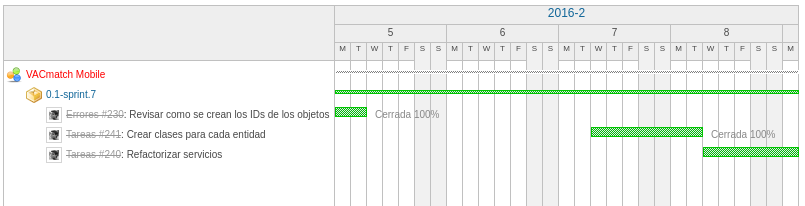
\includegraphics[width=\textwidth]{./img/gant_diagrams/07.png}
          \caption{Diagrama de Gant do sprint 7}
          \label{fig:gant07}
          \end{center}
        \end{figure}

    Para a realización desta iteración planificóuse un total de 22 horas e 
non se precisou ningunha hora extra para completar o traballo.

    \subsection{8ª iteración. Testing e integración continua}

      \subsubsection{Planificación e definición da iteración}
      A iteración transcorre entre os días 1 e 14 de Marzo.

      Decidiuse engadir tests unitarios para previr futuros erros e facilitar o 
mantemento da aplicación xa que en todo proxecto de certa embergadura, e máis 
en proxectos libres nos que calquera pode colaborar, é importante asegurar que 
os novos cambios que se engadan non xeneren problemas no funcionamento da 
aplicación.

      Relacionado con este tema tamén se planificou a integración do 
repositorio de código con unha ferramenta de integración continua que facilite 
a execución de este tipo de probas, en este caso Travis CI do que falaremos na 
Sección~\ref{sec:travis}.

      \subsubsection{Revisión e feedback}
      Durante esta iteración foi preciso publicar unha folla de ruta do 
proxecto no blog do mesmo, requisito fundamental solicitado pola organización 
do Concurso Universitario de Software Libre no que VACmatch se atopa inscrito 
dende o mes de Outubro aproximadamente.

      É por iso que se fixo unha entrada resumo para mostrar as tarefas 
existentes no Redmine do proxecto onde se realiza toda a xestión de 
incidencias así como se resaltaron os seguintes pasos a seguir no mesmo, como 
por exemplo, engadir a internacionalización ou permitir poñer en funcionamento 
a aplicación nun dispositivo móbil.

      \subsubsection{Tarefas e seguimento}

      As seguintes tarefas son as realizadas en esta iteración:

        \begin{description}
         \item [S8.1] Engadir tests aos servizos de Eventos, Persoas, Equipos e 
Actas.
         \item [S8.2] Engadir tests aos servizos de Auth, Árbitros e Sinaturas.
         \item [S8.3] Engadir integración continua con Travis CI.
         \item [S8.4] Engadir campos para confirmar contrasinal e código PIN ao 
crear un usuario.
        \end{description}

        \begin{figure}[h!]
          \begin{center}
          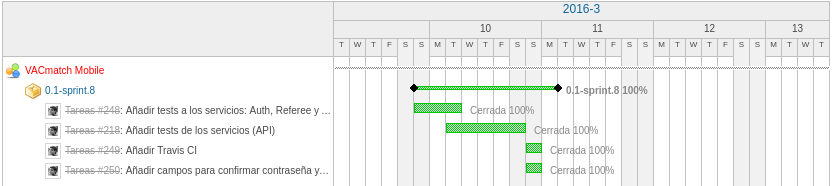
\includegraphics[width=\textwidth]{./img/gant_diagrams/08.png}
          \caption{Diagrama de Gant do sprint 8}
          \label{fig:gant08}
          \end{center}
        \end{figure}

        No diagrama da Figura~\ref{fig:gant08} pódese observar a evolución das 
tarefas ao longo do sprint que inicialmente tivo unha planificación de 37 horas 
pero finalmente alongouse 16 horas extra, obrigando a ampliar a xornada de 
traballo en 2 fines de semana a media xornada co obxectivo de non retrasar a 
execución das tarefas.

    \subsection{9ª e 10ª iteración. Inxección de dependencias}
    Motivado de novo pola inestabilidade e a falta de tempo dispoñible para 
realizar o proxecto, finalmente decidíuse integrar de novo estas dúas iteracións 
en unha.

      \subsubsection{Planificación e definición da iteración}
      Estas iteracións comezan o día 15 de Marzo e rematan o 25 de Abril.

      Detectáronse problemas en Travis xa que non detectaba erros nos tests 
polo que é o primeiro que había que corrixir.

      Tamén se decidíu crear unha barra de notificacións compartida para 
tódolos compoñentes da aplicación e engadíronse estados diferentes para as 
actas co fin de mostrar cando un encontro non comezou, cando se está a xogar e 
cando rematou.

      Pero a tarefa máis importante xurdíu ao aparecer un problema de 
dependencias circulares que obrigou a engadir unha factoría para realizar 
inxección de dependencias entre os servizos da aplicación xa que varios, 
dependían uns de outros.

      Finalmente planificouse tamén a corrección de diversos erros detectados 
na iteración anterior como o feito de non poder eliminar un xogador dun partido 
sen ter eliminados anteriormente os eventos que ten asignados en ese partido.

      \subsubsection{Revisión e feedback}
      Durante esta iteración non se publicou ningunha entrada no blog e 
tampouco se recibiron suxerencias.

      \subsubsection{Tarefas e seguimento}

      As tarefas definidas para esta iteración son as seguintes:

      \begin{description}
       \item [S10.1] Engadir textos de error na aplicación.
       \item [S10.2] Crear barra de notificacións para utilizar en calquera 
compoñente.
       \item [S10.3] Erro: Correxir problema de dependencias circulares.
       \item [S10.3.1] Engadir DAOs.
       \item [S10.3.2] Engadir Inxección de Dependencias.
       \item [S10.4] Erro: Mostrar que o partido rematóu na acta.
       \item [S10.4.1] Engadir estados na Acta.
       \item [S10.5] Erro: Como árbitro non debería poder convocar/borrar a un 
xogador que ten eventos asignados.
       \item [S10.6] Erro: Correxir erros varios derivados de engadir inxección 
de dependencias.
       \item [S10.7] Erro: Un evento de comezo de partido non se pode borrar si 
existe algún outro evento creado.
       \item [S10.8] Erro na xestión do estado da Acta.
       \item [S10.9] Erro: Travis CI non funciona correctamente
      \end{description}

        \begin{figure}[h!]
          \begin{center}
          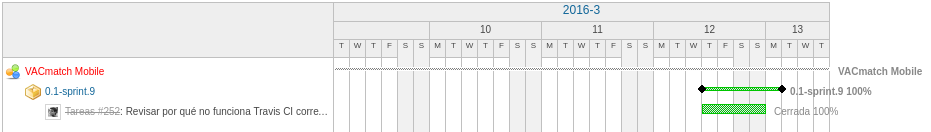
\includegraphics[width=\textwidth]{./img/gant_diagrams/09.png}
          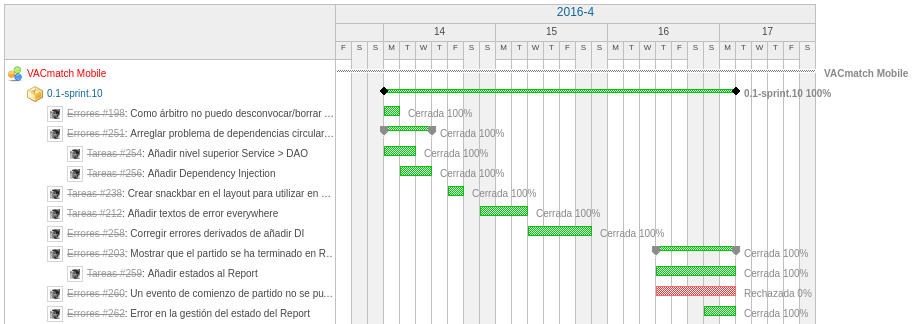
\includegraphics[width=\textwidth]{./img/gant_diagrams/10.png}
          \caption{Diagramas de Gant dos sprints 9 e 10}
          \label{fig:gant10}
          \end{center}
        \end{figure}

    A estimación inicial de horas para esta iteración foi de un total de 78, 
resultando unha vez máis, optimista e permitindo que a diferencia de horas 
coas reais, 66, poidesen ser reasignadas ao proxecto de VACmatch Web.

    \subsection{Release 0.2.0: Usabilidade en menús}

      \subsubsection{Planificación e definición da iteración}
      Esta iteración transcorre entre o día 25 de Abril e o 9 de Maio, 
unha iteración cunha única tarefa pero de abondo tamaño para 
cubrir a totalidade do sprint, centrada en engadir os enlaces que faltaban no 
menú lateral esquerdo e no superior dereito, certos botóns de retroceso así
como correxir diversos erros menores.

      \subsubsection{Concurso Universitario de Software Libre}
      Así mesmo, durante este iteración recibíuse o ``Premio al mejor proyecto 
de tecnologías móviles`` dentro do Concurso Universitario de Software Libre 
(CUSL), un concurso onde participaron máis de 75 estudantes de toda España con 
un total de 47 proxectos de código libre.

      Fomos invitados a participar na fase final que tivo lugar os días 5 e 6 
de Maio na Universidade de Sevilla na que presentar o proxecto ante 
representantes de diversas empresas de software libre españolas que tamén 
participaron con diversas charlas sobre os seus modelos de negocio e as 
vantaxes do software libre a nivel empresarial.

      Foi unha gran experiencia a compartida con tódolos finalistas e 
asistentes e, por suposto, os custes da viaxe foron subvencionados pola 
organización e o premio finalmente foi de 300 \euro{} en metálico.

    \begin{figure}[h!]
          \begin{center}
            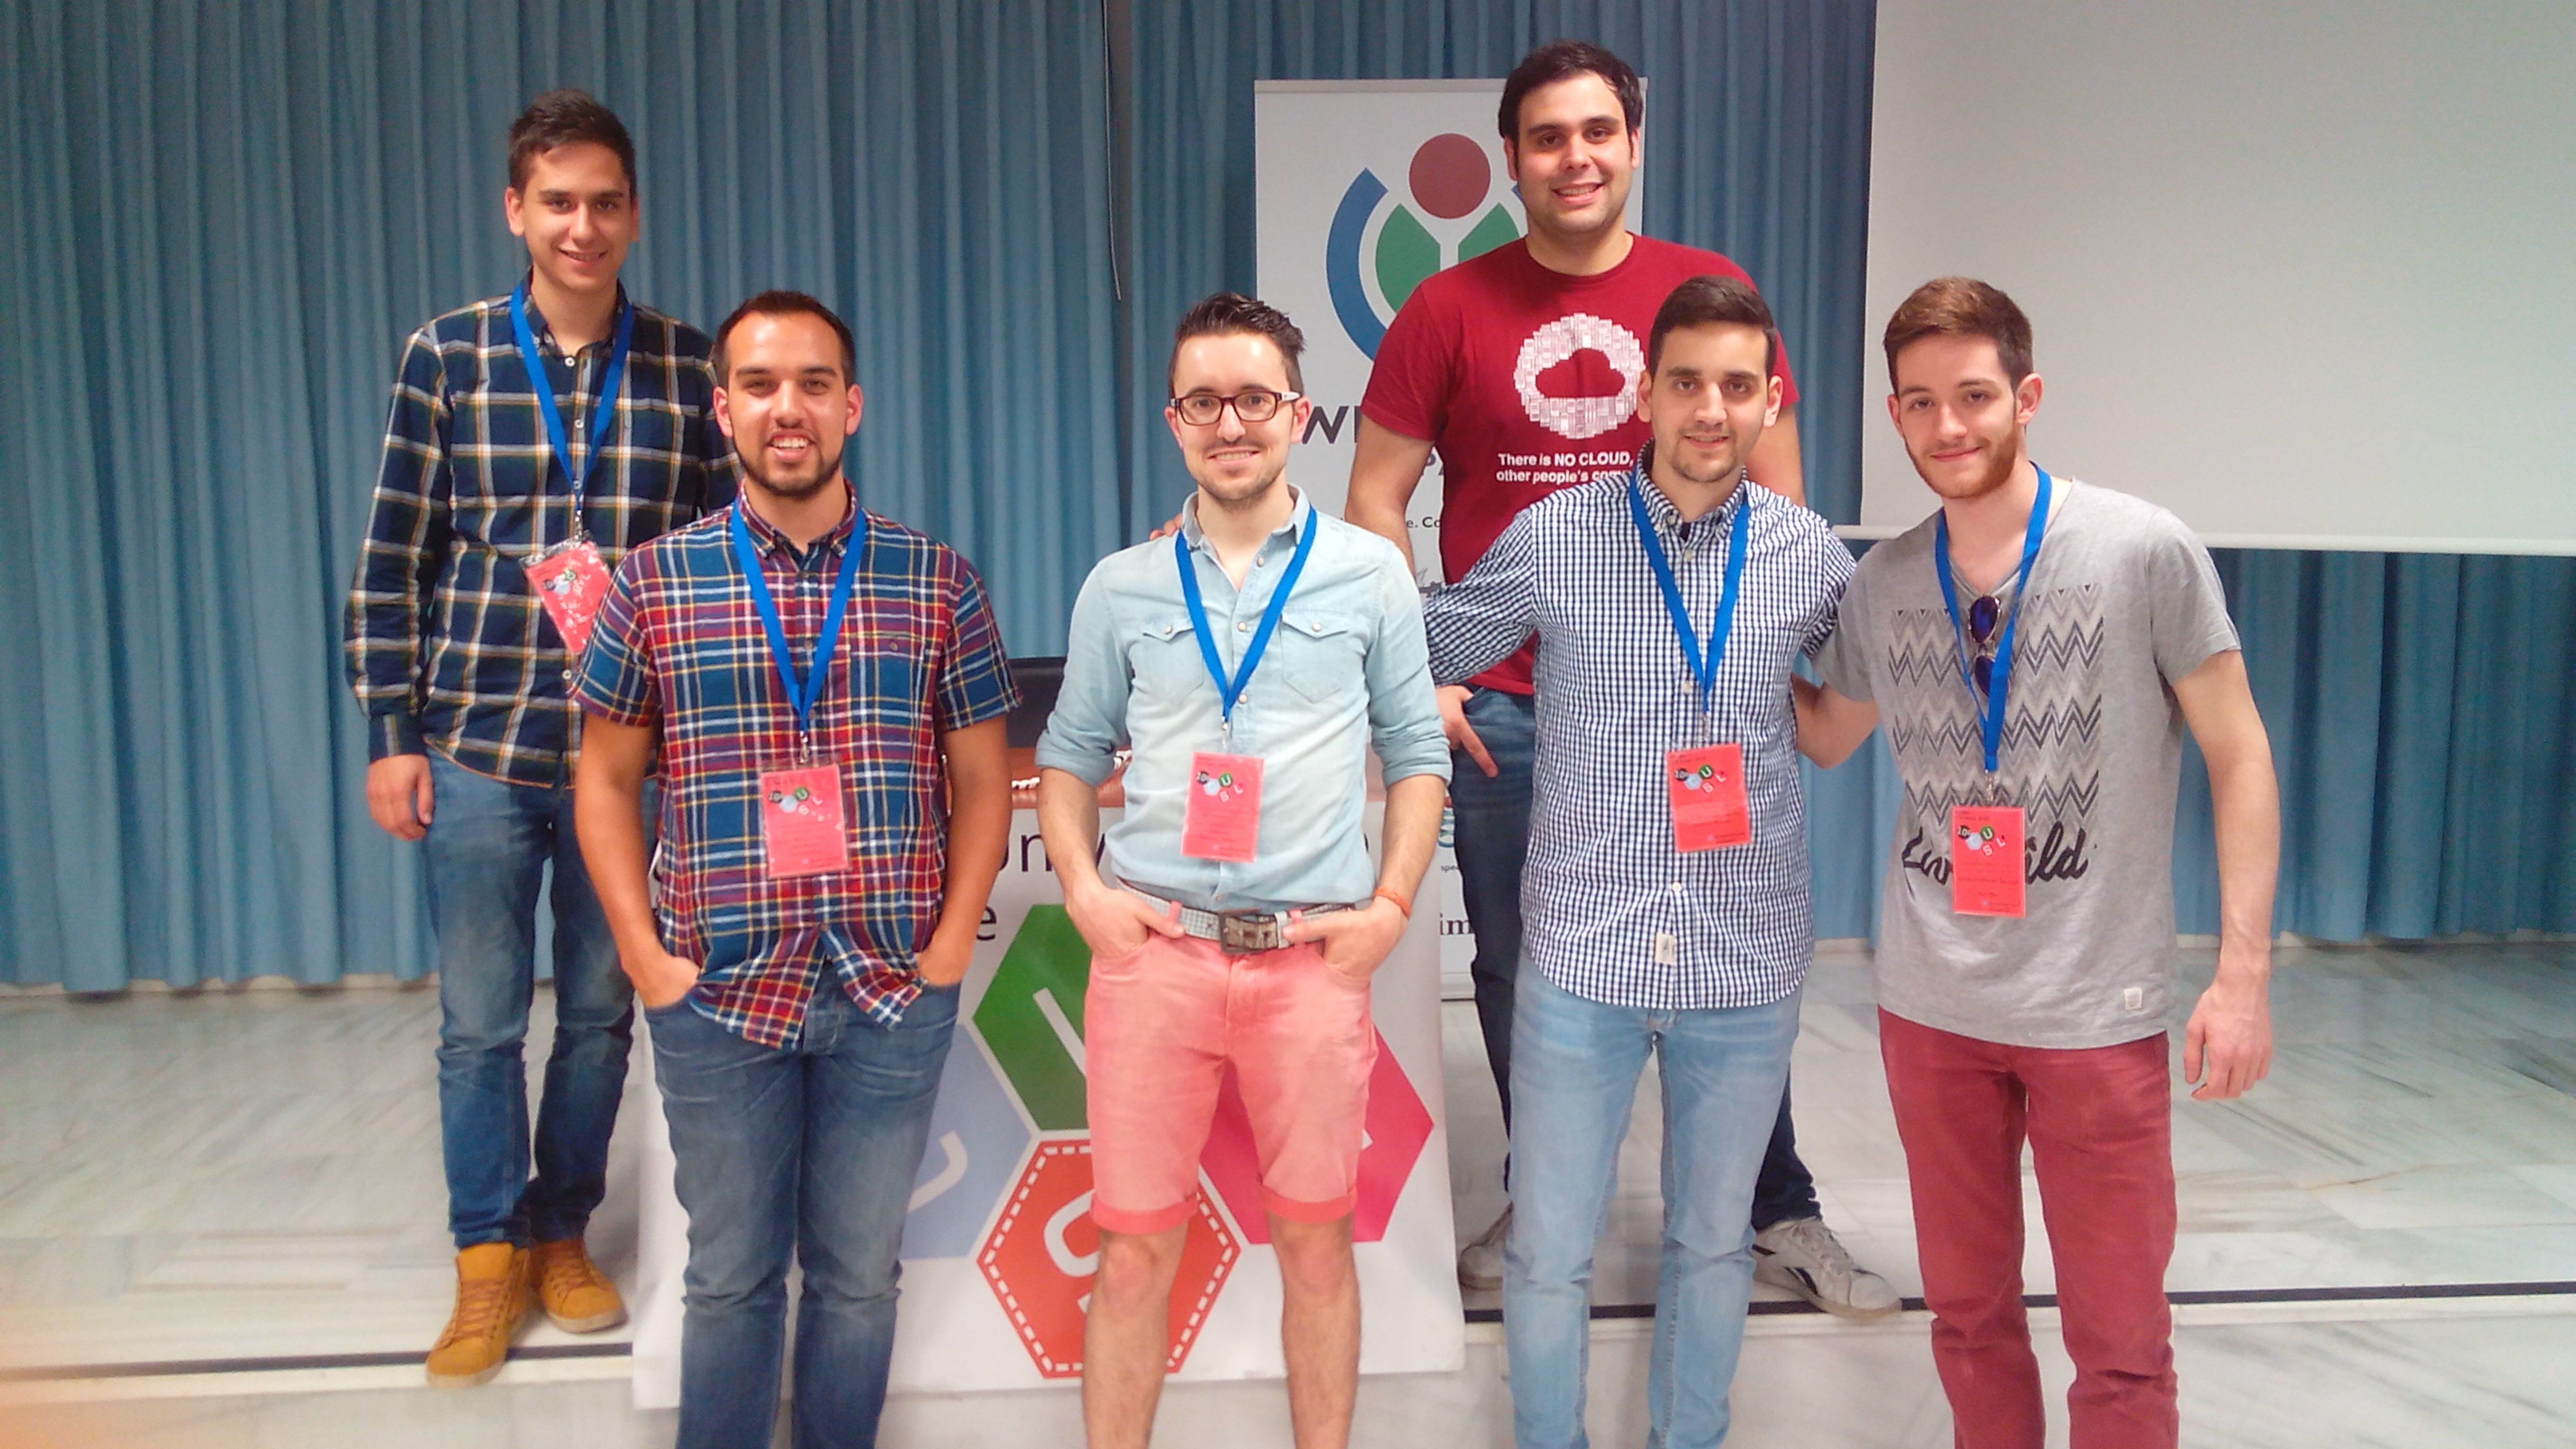
\includegraphics[width=0.8\textwidth]{./img/final_cusl.jpg}
            \caption{Finalistas CUSL.}
            \label{fig:cusl}
          \end{center}
    \end{figure}

      \subsubsection{Revisión e feedback}
      Aproveitando a participación no CUSL obtivéronse múltiples consexos e 
suxerencias, sobre todo en temas concretos de desenvolvemento xa que o xurado 
realizou unha profunda revisión do código da aplicación.

      Entre elas destaca sobre todo a proposta de tratar de cambiar os 
múltiples \lstinline{Callbacks} por \lstinline{Promises} de Javascript así como 
outros consellos para facilitar o mantemento do código como evitar encadear 
demasiados métodos.

      Paralelamente publicouse unha entrada no blog no que comentar os diversos 
problemas xurdidos que obligaron a engadir inxección de dependencias así como a 
enorme refactorización de código levada a cabo para introducir tests 
automáticos e integración continua.

      \subsubsection{Tarefas e seguimento}

      Únicamente se realizou unha tarefa durante este período:

        \begin{description}
          \item [S0.2.0-1] Revisar os links nos menús e engadir información.
        \end{description}

        \begin{figure}[h!]
          \begin{center}
          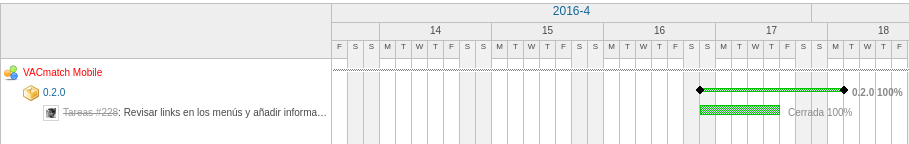
\includegraphics[width=\textwidth]{./img/gant_diagrams/020.png}
          \caption{Diagramas de Gant da release 0.2.0}
          \label{fig:gant20}
          \end{center}
        \end{figure}

     Esta tarefa tivo unha planificación moito máis reducida do habitual (16 
horas) xa que ao resultar finalistas no CUSL, debeuse viaxar a Sevilla durante 
un total de tres días.

     Finalmente o tempo invertido no desenvolvemento foi un total de 14 
horas, aproveitando as 2 horas restantes para preparar a 
presentación para o concurso.

    \subsection{Release 0.2.1: I18n e app híbrida}

      \subsubsection{Planificación e definición da iteración}
      Esta iteración comeza o día 9 e remata o 24 Maio.

      A tarefa de maior tamaño que se planificou nesta iteración foi a 
internacionalización coa librería React Intl xa que supón modificar tódalas 
vistas da aplicación.

      Posteriormente engadíuse Apache Cordova para permitir crear aplicacións 
híbridas que funcionen en múltiples sistemas operativos móbiles e por suposto, 
tamén se incluíu no repositorio de código, a documentación sobre cómo arrancar 
unha base de datos CouchDB para utilizar como backend e sobre cómo realizar a 
compilación da aplicación para executar nun sistema operativo móbil.

      \subsubsection{Revisión e feedback}
      Durante esta etapa tampouco se recibíu feedback nin se escribiu ningunha 
entrada no blog.

      \subsubsection{Tarefas e seguimento}
        \begin{description}
        \item [S0.2.1-1] Engadir internacionalización.
        \item [S0.2.1-2] Crear app híbrida con Apache Córdova.
        \end{description}

        \begin{figure}[h!]
          \begin{center}
          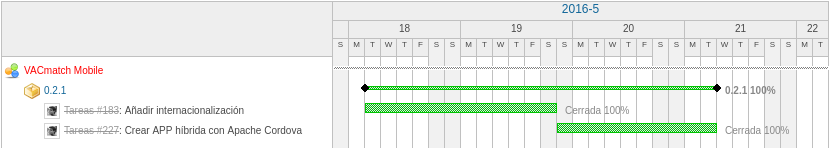
\includegraphics[width=\textwidth]{./img/gant_diagrams/021.png}
          \caption{Diagramas de Gant da release 0.2.1}
          \label{fig:gant21}
          \end{center}
        \end{figure}

        A duración estimada da iteración foi de 36 horas e finalmente 
realizouse en 1 hora máis do previsto que foi imputada como hora extra para non 
retrasar o desenvolvemento.

    \subsection{Release 0.2.2: Finalización da memoria e revisión de erros}

      \subsubsection{Planificación e definición da iteración}
      Esta última iteración comeza o 25 de Maio e exténdese finalmente ata o 
día 19 de xuño.

      Céntrase principalmente en engadir certas vistas da 
aplicación como a de ''Acerca de`` ou a de configuración así como múltiples 
detalles visuais como engadir unha transición mentras os datos non se atopan 
cargados e solucionar diversos erros atopados na aplicación.

      Así mesmo tamén se adicou un tempo considerable á finaliación da memoria.

      \subsubsection{Revisión e feedback}
      Durante esta iteración coñeceuse que VACmatch foi invitado a 
participar na fase final do ''Certamen de Proyectos Libres de la Universidad de 
Granada`` co presente proxecto pero non foi posible asistir polo que se decidiu 
enviar un vídeo para realizar a presentación e polo tanto tampouco se puido 
obter feedback.

      \subsubsection{Tarefas e seguimento}

      Ao longo da iteración realizáronse as seguintes tarefas:

        \begin{description}
        \item [S0.2.2-1] Error ao engadir un evento, cámbiase o nome dos equipos
        \item [S0.2.2-2] Error ao tratar de asinar un acta como árbitro e como 
xogador creado na app móbil
        \item [S0.2.2-3] Eliminar páxina de home
        \item [S0.2.2-4] Non se engaden ao menú lateral esquerdo en ningún 
momento a lista de actas
        \item [S0.2.2-5] Un xogador debe poder asinar un acta incluso si é 
creado manualmente na acta 
        \item [S0.2.2-6] Os links do menú lateral esquerdo non funcionan
        \item [S0.2.2-7] [Memoria] Apendices
        \item [S0.2.2-8] [Memoria] Conclusións
        \item [S0.2.2-9] [Memoria] Deseño e implementación
        \item [S0.2.2-10] [Memoria] Planificación e seguimento
        \item [S0.2.2-11] [Memoria] Revisión xeral
        \item [S0.2.2-12] Só mostrar/editar as actas do usuario que está 
logueado
        \end{description}

        A estimación inicial para a realización desta iteración foi dun total 
de 91 horas, cumpríndose correctamente e dispoñendo finalmente de 10,5 horas 
libres para adicar a aprender tecnoloxías que é posible que se utilicen nun 
futuro cercano como é o caso de Docker, para realizar entregas contínuas.

        Na Figura~\ref{fig:gant22} pódese observar o Diagrama de Gant da 
iteración.

        \begin{figure}[h!]
          \begin{center}
          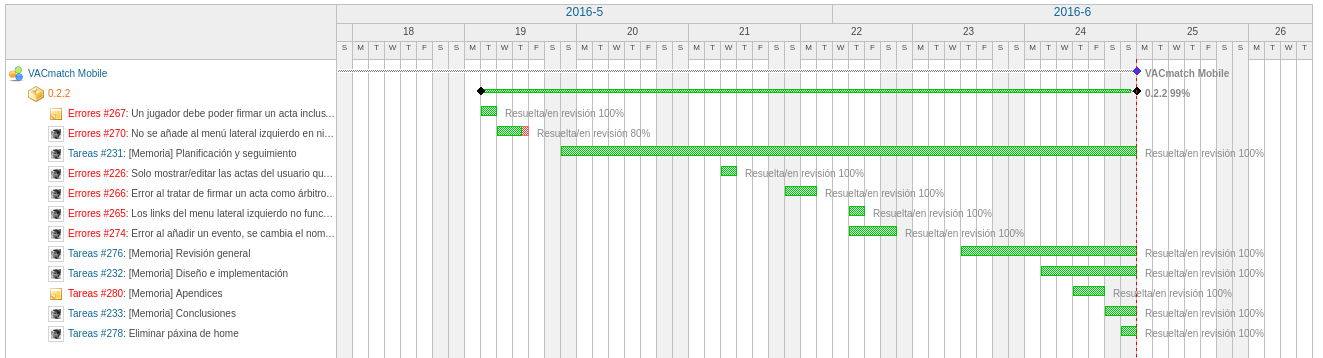
\includegraphics[width=\textwidth]{./img/gant_diagrams/022.png}
          \caption{Diagramas de Gant da release 0.2.2}
          \label{fig:gant22}
          \end{center}
        \end{figure}

%%% Local Variables:
%%% mode: latex
%%% TeX-master: "../root"
%%% End:
